\chapter{Experimentos e Resultados Preliminares}\label{cap:experimentos}

\section{Base de dados}

A base de dados (imagens) utilizada advém do projeto GEOMA \cite{geoma}, financiado pelo Instituto de Pesquisas Espaciais (INPE). Trata-se de imagens coloridas, codificadas em JPEG e com 640 pixels de largura por 480 pixels de altura. A base é composta por fotografias ortogonais ao relevo (como pode ser visto na figura \ref{fig:amostra}), de altitudes variadas e tiradas a partir de aeronaves tripuladas, durante o trajeto entre diversas cidades da região amazônica.

No momento do início dos experimentos deste trabalho, estas imagens tiradas de aviões tripulados eram as únicas disponíveis publicamente. Podemos considerá-las válidas por terem sido tiradas em altitude de voo compatível com as missões de VANTs de vigilância, entre 900 e 1.100 metros do solo. Como este trabalho tem como objetivo utilizar apenas câmeras de espectro visível, são dispensáveis comparações de sensores com VANTs que eventualmente possuam sonar, câmeras infravermelho ou outros tipos de sensores.

\begin{figure}[h]
  \centering
  \begin{subfigure}[b]{0.3\textwidth}
    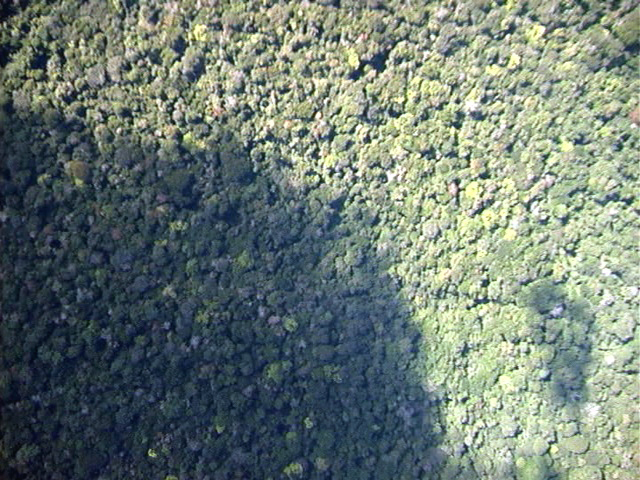
\includegraphics[width=\textwidth]{imgs/amostra1}
  \end{subfigure}%
  ~
  \begin{subfigure}[b]{0.3\textwidth}
    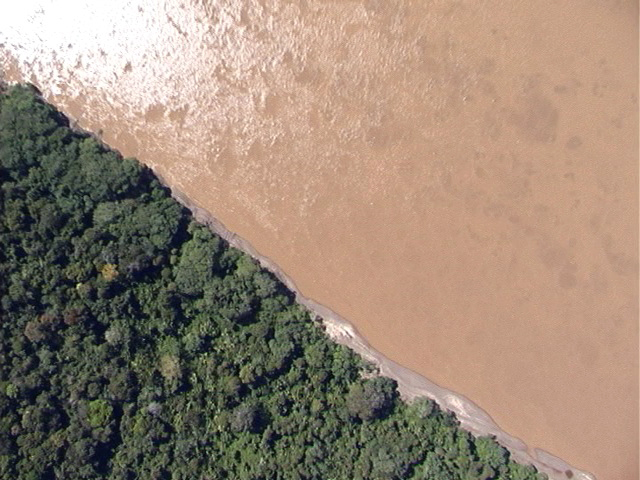
\includegraphics[width=\textwidth]{imgs/amostra2}
  \end{subfigure}%
  ~
  \begin{subfigure}[b]{0.3\textwidth}
    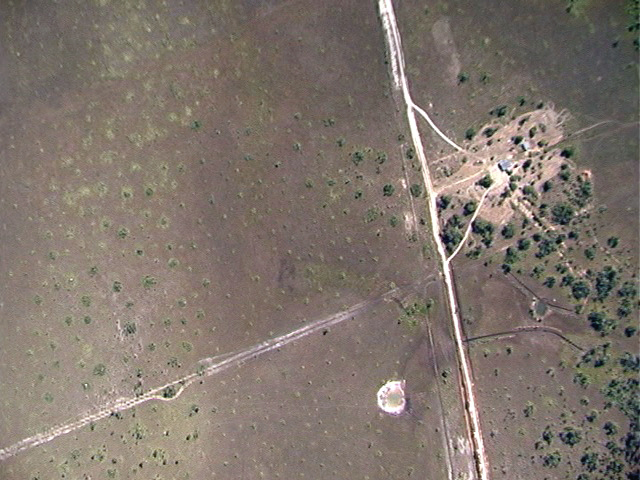
\includegraphics[width=\textwidth]{imgs/amostra3}
  \end{subfigure}%
  \caption{Amostras da base de dados}
  \label{fig:amostra}
\end{figure}

A base possui um total de 3.044 imagens, com dimensão total de 1,02 Gigabytes de dados. Cerca de 150 imagens foram utilizadas nos experimentos até o momento, visto que um grande esforço precisa ser despendido na classificação manual das imagens em todas as etapas do experimento, consumindo um tempo considerável.

Para facilitar a classificação manual foi construída uma ferramenta gráfica que permite ao usuário segmentar e classificar as regiões das imagens de acordo com as classes disponíveis (figura \ref{fig:visualClassifier}). A saída deste aplicativo é uma coleção, para cada imagem, de informações sobre bordas das regiões e a classificação de cada pixel. Posteriormente essas informações serão confrontadas com o resultado da segmentação e primeiro nível de classificação da solução.

\begin{figure}[h]
  \centering
  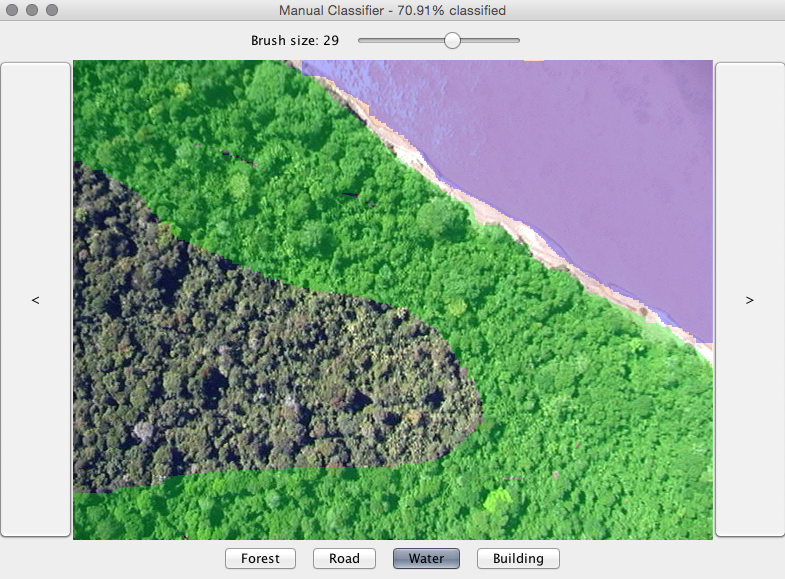
\includegraphics[width=0.7\textwidth]{imgs/visualClassifier}
  \caption{Ferramenta para segmentação e classificação manual das imagens em regiões}
  \label{fig:visualClassifier}
\end{figure}

\section{Segmentação}

Para determinar qual dos algoritmos de segmentação levantados na pesquisa bibliográfica teria melhor desempenho na base de dados utilizada neste trabalho, todos foram implementados ou adaptados. Os algoritmos foram testados no conjunto inicial de 150 imagens e comparados com a segmentação manual realizada nas mesmas imagens.

Para avaliar as diferentes segmentações, o método introduzido por \citeonline{martin:2001} foi utilizado. Este método consiste na sobreposição de regiões e comparação de informações sobre localização e orientação dos elementos de borda (\textit{edgels}).

Os resultados do experimento são apresentados na tabela \ref{tab:experimentoSegmentacao}:

\begin{table}[h]
\ABNTEXfontereduzida
\centering
\begin{tabulary}{\linewidth}{|L|R|R|}
\hline
\textbf{Algoritmo} & \textbf{Acurácia} & \textbf{Tempo/imagem} \\ \hline
Mean-shift  & 97,2\% & 6,39 s \\ \hline
JSEG        & 96,3\% & 14,82 s \\ \hline
MSEG        & 94,1\% & 0,33 s \\ \hline
SRM         & 91,9\% & 4,66 s \\ \hline
FSEG        & 81,4\% & 13,91 s \\ \hline
gPb-owt-ucm & 72,2\% & 237,32 s \\ \hline
\end{tabulary}
\caption{Comparação de métodos de segmentação em parte da base de imagens deste trabalho, ordenados por acurácia}
\label{tab:experimentoSegmentacao}
\end{table}

O algoritmo Mean-shift, além de ter conseguido a melhor precisão na nossa base de dados, conseguiu um bom desempenho de tempo. Com isso, pudemos determinar que ele será o algoritmo utilizado no trabalho, para a segmentação inicial das imagens.

O método JSEG conseguiu uma precisão bastante próxima do Mean-shift e será considerado uma alternativa, embora o tempo de segmentação deste algoritmo seja consideravelmente maior. A imagem \ref{fig:comparacaoSegmentacao} mostra a saída de alguns dos métodos testados, para fins de comparação visual.

\begin{figure}[htb]
	\centering
	\begin{minipage}[l]{0.51\linewidth}
		\begin{subfigure}[b]{\linewidth}
			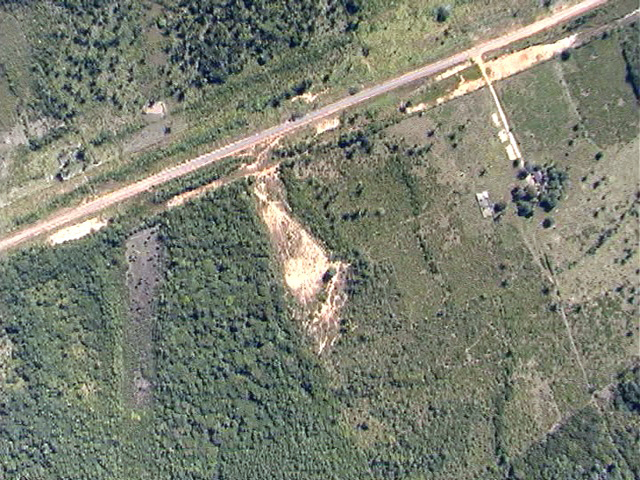
\includegraphics[width=\linewidth]{imgs/seg_original}
			\caption{Imagem original}
		\end{subfigure}%
	\end{minipage}
	\begin{minipage}[r]{0.48\linewidth}
		\begin{subfigure}{.47\linewidth}
			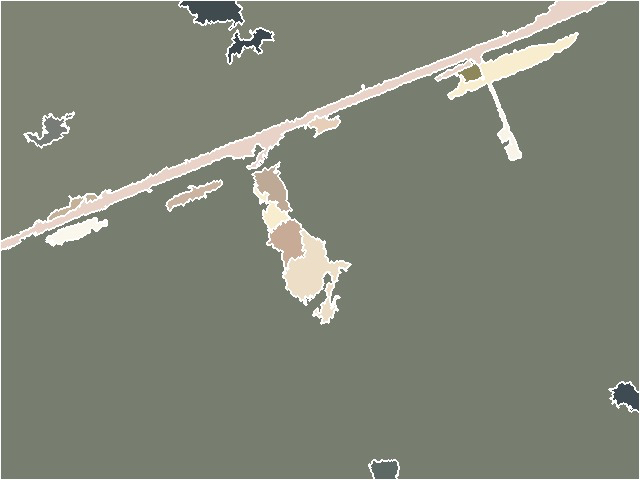
\includegraphics[width=\linewidth]{imgs/seg_meanshift}
			\caption{Mean-shift}
		\end{subfigure}
		\begin{subfigure}{.47\linewidth}
			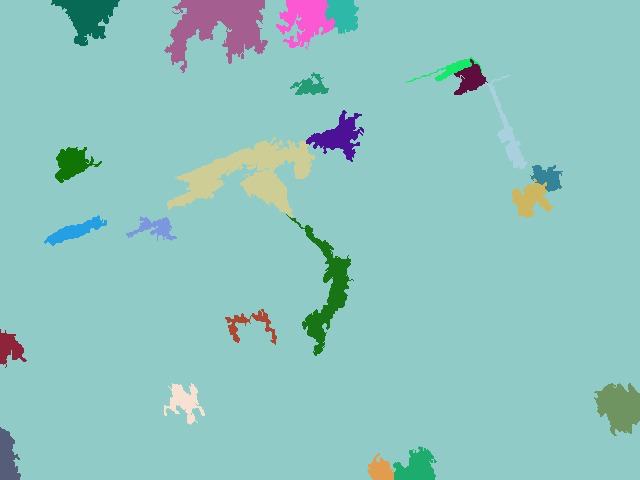
\includegraphics[width=\linewidth]{imgs/seg_mseg}
			\caption{MSEG}
		\end{subfigure}%
		\\
		\begin{subfigure}{.47\linewidth}
			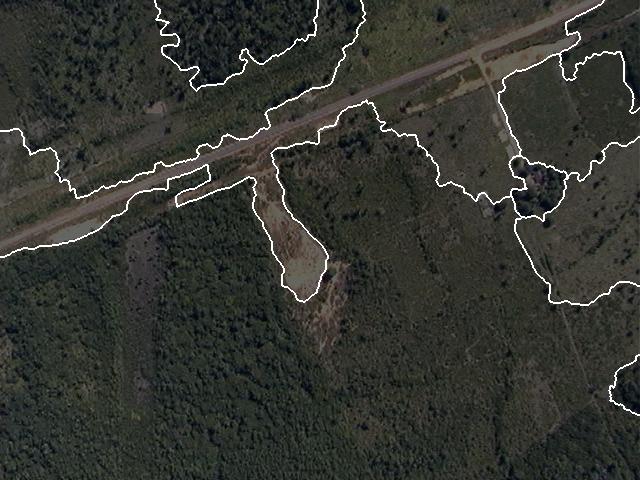
\includegraphics[width=\linewidth]{imgs/seg_jseg}
			\caption{JSEG}
		\end{subfigure}
		\begin{subfigure}{.47\linewidth}
			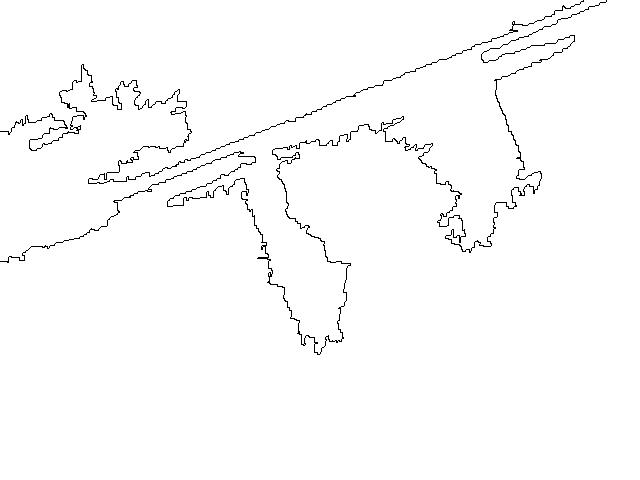
\includegraphics[width=\linewidth]{imgs/seg_srm}
			\caption{SRM}
		\end{subfigure}%
	\end{minipage}
	\caption{Comparação visual de métodos de segmentação}
	\label{fig:comparacaoSegmentacao}
\end{figure}


Adicionalmente, experimentos foram realizados com técnicas de classificação. O objetivo era saber se poderíamos utilizar apenas uma etapa para realizar segmentação e o primeiro nível de classificação. Os resultados foram abaixo do que se consegue na etapa de segmentação isolada. Os resultados foram publicados no \textit{$10^th$ International Conference on Computer Vision Theory and Applications} e o artigo \cite{cavalcanti:2015} completo pode ser visto no apêndice \ref{cap:apendice}.

Para fins de comparação, os resultados deste segundo experimento são apresentados na tabela \ref{tab:experimentoArtigo}. O tempo de execução da classificação para cada imagem no artigo publicado ignora o tempo de extração de características da imagem. Para uma comparação correta com os métodos de segmentação experimentados anteriormente, esse tempo gasto em extração de características foi acrescido na tabela desta seção.

\begin{table}[h]
\ABNTEXfontereduzida
\centering
\begin{tabulary}{\linewidth}{|L|R|R|}
\hline
\textbf{Algoritmo} & \textbf{Acurácia} & \textbf{Tempo/imagem} \\ \hline
Random forest  & 96,0\% & 12,72 s \\ \hline
KNN            & 92,6\% & 22,89 s \\ \hline
Naive Bayes    & 92,8\% & 8,36 s \\ \hline
Decision tree  & 82,2\% & 14,49 s \\ \hline
\end{tabulary}
\caption{Comparação de métodos de classificação para segmentação das imagens em uma única etapa, ordenados por acurácia}
\label{tab:experimentoArtigo}
\end{table}


\section{Classificações de regiões}

Para o primeiro nível de classificação, que se resume a definir os tipos de terrenos das regiões encontradas na segmentação, um experimento com métodos bastante difundidos de aprendizagem de máquina foi realizado.

Utilizando as técnicas de K vizinhos mais próximos (KNN), máquinas de vetores de suporte (SVM) e árvores de decisão, um experimento foi conduzido em uma parte da base de dados. As mesmas 150 imagens do experimento de segmentação anteriormente apresentado foram utilizadas.

Primeiramente, todas as imagens foram segmentadas utilizando o método Mean-shift, por ter obtido o melhor desempenho no experimento de segmentação anterior. Cada região encontrada nesta segmentação foi devidamente classificada manualmente, e suas características foram extraídas. A partir desse ponto bases de dados de treinamento e validação supervisionadas foram criadas, onde cada região segmentada representava uma amostra de treinamento ou validação.

As características extraídas para cada região foram:
\begin{itemize}
	\item Cor média para os canais vermelho, verde e azul;
	\item Histograma dos canais vermelho, verde e azul;
	\item Tom de cinza médio;
	\item Histograma de tons de cinza.
\end{itemize}

O total de 7.111 amostras foram classificadas, onde 4.694 (66\%) foram utilizadas como amostras de treinamento e 2.417 (33\%) foram utilizadas como amostras de validação. O método SVM teve desempenho ligeiramente superior aos demais, como pode ser visto na tabela \ref{tab:experimentoClassificacao1}, que apresenta os resultados de acurácia, precisão, e revocação para os métodos analisados.

\begin{table}[h]
\ABNTEXfontereduzida
\centering
\begin{tabulary}{\linewidth}{|L|R|R|R|}
\hline
\textbf{Método} & \textbf{Acurácia} & \textbf{Precisão} & \textbf{Revocação} \\ \hline
SVM               & 89,19\% & 0,927 & 0,864 \\ \hline
KNN               & 88,51\% & 0,912 & 0,863 \\ \hline
Árvore de decisão & 87,09\% & 0,842 & 0,859 \\ \hline
\end{tabulary}
\caption{Comparação de métodos de classificação para regiões segmentadas das imagens, ordenados por acurácia}
\label{tab:experimentoClassificacao1}
\end{table}

Embora os resultados tenham sido promissores, ainda há bastante espaço para melhoria. Apenas características de cor e luminância foram exploradas, portanto, características de textura, morfologia e borda ainda precisam ser avaliadas.

\section{Próximos passos}

Para os próximos meses de pesquisa, diversas características serão extraídas e avaliadas para o primeiro nível de classificação:

\begin{itemize}
	\item Bordas;
	\item Textura;
	\item Morfologia;
	\item Bag of visual words
	\item Vizinhança de regiões.
\end{itemize}

Além disso, técnicas ensembles de classificadores também serão avaliados e comparados com os resultados atuais.

Para a fase final de classificação, será feito um levantamento de características e algoritmos de classificação para a detecção de elementos anômalos dentro das regiões segmentadas. Nesta fase serão explorados classificadores unitários (\textit{one-class classifiers}), visto que a literatura relata bons resultados com este tipo de classificador para detecção de anomalias e \textit{outliers}. Após estes experimentos, todo o fluxo de classificação será reavaliado, a fim de otimizar a taxa de aprendizado e generalização dos classificadores.

Por fim, o volume final da dissertação de mestrado será composto, levando em consideração os melhores resultados dos experimentos. Artigos também serão feitos e submetidos, refletindo partes relevantes da pesquisa e seus resultados.
